\documentclass[14pt,a4paper]{report}
\usepackage[utf8]{inputenc}
\usepackage{graphicx}
\usepackage{subcaption}
\usepackage{tikz}
\usepackage{caption}
\usepackage{float}
\usepackage[affil]{authblk}
\usepackage{pgfplots,caption}
\usepackage{titlepic}
\pgfplotsset{compat=1.9}

\title{\textbf{Fibonacci Heaps}}
% \titlepic{
\includegraphics[width=\textwidth]{Buet-Vector-Logo.png}}
\author{\textbf{Saem Hasan}\\1705027\\\textbf{Samira}\\1705028}

\affil{Department of Computer Science \& Engineering}
\affil{Bangladesh University of Engineering and Technology}
\date{\today}

\begin{document}

\maketitle
\tableofcontents
\pagebreak

\chapter{Introduction}
Fibonacci heap is a data structure which is applied on a set of items. Fibonacci heap is similar to Binomial heap. Fibonacci heap is used where merging heap is costly. In other heap , merging takes O(n) time where fibonacci heap takes O(1). Other than that it has some other operation like insertion, Decrease key, Union, Delete, Find minimum ,Extract min. Fibonacci heap has a less rigid structure than other heaps.It lazily consolidates until the next Extract-min operation. Fibonacci is faster for network optimization problem.
\chapter{Binary Heap}
A binary heap is a heap data structure that takes the form of a binary tree. Binary heaps are a common way of implementing priority queues. \\ \\
A binary heap is defined as a binary tree with two additional constraints: 
\begin{itemize}
    \item \textbf{Structural property:} A binary heap is an almost complete binary tree. It is complete on all levels except the last. 
    \item \textbf{Order property:} A binary heap maintains a minimum/maximum heap order property. The minimum/maximum key is stored in the root. The key stored in each node is either less than or equal to or greater than or equal to the keys of the node's children. 
\end{itemize}

% \centering
\begin{figure}[H]
    \centering
    \begin{tikzpicture}[
roundnode/.style={circle, draw=black!60, fill=black!20, very thick, minimum size=3mm, inner sep=1pt,}
]
    
    \node [roundnode] (b1) at (0,-0.9) {14};
    
    \node [roundnode] (c1) at (-0.6,-2.1) {26};
    \node [roundnode] (c2) at (0.6,-2.1) {31};
    
    \node [roundnode] (d1) at (-1.2,-3.3) {44};
    \node [roundnode] (d2) at (0.0,-3.3) {35};
    
    \draw (b1) edge (c1);
    \draw (b1) edge (c2);
    \draw (c1) edge (d1);
    \draw (c1) edge (d2);
    \end{tikzpicture} 
    \caption{Binary Heap}
    \label{fig:my_label}
\end{figure}
   
   
   
\section{Binary Heap: Properties}
    \begin{itemize}
        \item Binary heap stores maximum/minimum key in the root.
        \item Binary heap maintains a pointer to the root node.
        \item Each node maintains pointers to it's child node.
        \item Binary heap with n elements has floor(logn) height where n equals to the number of nodes of the heap.
    \end{itemize}
    
    \begin{figure}
        \centering
        
        \begin{tikzpicture}[
roundnode/.style={circle, draw=black!60, fill=black!20, very thick, minimum size=3mm, inner sep=1pt,}
]
    \node [roundnode] (a1) at (0, 0) {10};
    
    \node [roundnode] (b1) at (-2,-0.9) {14};
    \node [roundnode] (b2) at (2,-0.9) {19};
    
    \node [roundnode] (c1) at (-2.6,-2.1) {26};
    \node [roundnode] (c2) at (-1.4,-2.1) {31};
    \node [roundnode] (c3) at (1.4,-2.1) {42};
    \node [roundnode] (c4) at (2.6,-2.1) {27};
    
    \node [roundnode] (d1) at (-3.2,-3.3) {44};
    \node [roundnode] (d2) at (-2.0,-3.3) {35};
    
    
    \draw (a1) edge (b1);
    \draw (a1) edge (b2);
    \draw (b1) edge (c1);
    \draw (b1) edge (c2);
    \draw (b2) edge (c3);
    \draw (b2) edge (c4);
    \draw (c1) edge (d1);
    \draw (c1) edge (d2);
    \draw[<->] (-4,0) edge (-4,-3.3) node[left] {logn};;
   % \draw[<-] (0.5,0) edge (2,0)
    \draw [thick,<-](0.5,0) to (2,0,0);
    \end{tikzpicture}    
    
        \caption{Binary Heap}
        \label{fig:my_label}
    \end{figure}
    
    

\section{Building Binary Heap}
To build a binary heap with n keys, we can take two approaches:
\begin{enumerate}
    \item We can call insert operation of binary heap for n keys. Each insert operation takes O(logn) time. Then to build a heap, we have to call insert operation n times.
    \begin{itemize}
        \item Running time to build a heap by calling insert operation : O(nlogn)
    \end{itemize}
    
    \item We can construct a binary tree. For i=n to 1, we can repeatedly exchange the key in node i with it's smaller/larger child until the heap property is achieved. We can do this in linear time. 
    \begin{itemize}
        \item Running time to build a heap by constructing a binary tree : O(n)
    \end{itemize}
\end{enumerate}
    
\section{Merge Binary Heaps}
There is no easy solution to merge two binary heaps. We can take a approach. We can merge all keys of two heaps and then we can call build heap operation. Build heap operation takes O(n) time. 

\bigskip

\begin{figure}[H]
    \centering
        \begin{tikzpicture}[
roundnode/.style={circle, draw=black!60, fill=black!20, very thick, minimum size=3mm, inner sep=1pt,}
]
   
    \node [roundnode,label=right:H1] (b1) at (-2,-0.9) {14};
    \node [roundnode,label=right:H2] (b2) at (2,-0.9) {19};
    
    \node [roundnode] (c1) at (-2.6,-2.1) {26};
    \node [roundnode] (c2) at (-1.4,-2.1) {31};
    \node [roundnode] (c3) at (1.4,-2.1) {42};
    \node [roundnode] (c4) at (2.6,-2.1) {27};
    
    \node [roundnode] (d1) at (-3.2,-3.3) {44};
    \node [roundnode] (d2) at (-2.0,-3.3) {35};
    
    \draw (b1) edge (c1);
    \draw (b1) edge (c2);
    \draw (b2) edge (c3);
    \draw (b2) edge (c4);
    \draw (c1) edge (d1);
    \draw (c1) edge (d2);
    
    \end{tikzpicture}    

    \caption{Merge Heaps}
    \label{fig:my_label}
\end{figure}

\bigskip

\begin{figure}[H]
    \centering
    
    
   \begin{tikzpicture}[
roundnode/.style={circle, draw=black!60, fill=black!20, very thick, minimum size=3mm, inner sep=1pt,}
]

    \node [roundnode] (b1) at (0,0) {14};
    \node [roundnode] (b2) at (4.0,0) {19};
    
    \node [roundnode] (c1) at (0.8,0) {26};
    \node [roundnode] (c2) at (1.6,0) {31};
    \node [roundnode] (c3) at (4.8,0) {42};
    \node [roundnode] (c4) at (5.6,0) {27};
    
    \node [roundnode] (d1) at (2.4,0) {44};
    \node [roundnode] (d2) at (3.2,0) {35};

\end{tikzpicture}
 
    
    
    \caption{All elements of H1 \& H2}
    \label{fig:my_label}
\end{figure}


   
\bigskip

\begin{figure}[H]
    \centering
    
    
\begin{tikzpicture}[
roundnode/.style={circle, draw=black!60, fill=black!20, very thick, minimum size=3mm, inner sep=1pt,}
]
\node [roundnode,label=right:H] (b1) at (0,0) {14};
    
    \node [roundnode] (c1) at (-2,-0.9) {26};
    \node [roundnode] (c2) at (2,-0.9) {19};
    
    
    \node [roundnode] (d1) at (-2.6,-2.1) {27};
    \node [roundnode] (d2) at (-1.4,-2.1) {35};
    \node [roundnode] (d3) at (1.4,-2.1) {31};
    \node [roundnode] (d4) at (2.6,-2.1) {42};
    
    \node [roundnode] (e1) at (-3.2,-3.3) {44};
    
    \draw (b1) edge (c1);
    \draw (b1) edge (c2);
    \draw (c1) edge (d1);
    \draw (c1) edge (d2);
    \draw (c2) edge (d3);
    \draw (c2) edge (d4);
    \draw (d1) edge (e1);
    \end{tikzpicture}

    
    \caption{Merged Heap}
    \label{fig:my_label}
\end{figure}

\bigskip

\begin{itemize}
    \item Running time to merge two heaps: O(n)
\end{itemize}

\chapter{Mergeable Heaps}
We can merge two heaps by taking all keys of two heaps and calling build heap operation. We can do this in O(n) time. But we can merge two heaps faster than O(n). There are two well-known mergeable heap data structures:
\begin{enumerate}
    \item Binomial Heap
    \item \textbf{Fibonacci Heap}
\end{enumerate}
In this report, we will mainly focus on Fibonacci Heap.
\chapter{Binomial Heap}
Binomial Heap is a collection of binomial trees. There is at most one binomial tree of order in a binomial heap. 
\begin{figure}[h]
    \centering
    
    \begin{tikzpicture}
      \filldraw [black] (0,0) circle (2pt);
      
      \filldraw [black,xshift=1cm] (0,0) circle (2pt);
      \filldraw [black,xshift=1cm, yshift=-1cm] (0,0) circle (2pt);
      \draw[thick] (1,0) -- (1,-1);
      
      \filldraw [black,xshift=2cm] (0,0) circle (2pt);
      \filldraw [black,xshift=2cm, yshift=-1cm] (0,0) circle (2pt);
      \draw[thick] (2,0) -- (2,-1);
      \filldraw [black,xshift=3cm, yshift=-1cm] (0,0) circle (2pt);
            \draw[thick] (2,0) -- (3,-1);
      \filldraw [black,xshift=3cm, yshift=-2cm] (0,0) circle (2pt);
      \draw[thick] (3,-1) -- (3,-2);
      
      \filldraw [black,xshift=4cm] (0,0) circle (2pt);
      \filldraw [black,xshift=4cm, yshift=-1cm] (0,0) circle (2pt);
       \draw[thick] (4,0) -- (4,-1);
      \filldraw [black,xshift=5cm, yshift=-1cm] (0,0) circle (2pt);
       \draw[thick] (4,0) -- (5,-1);
       
      \filldraw [black,xshift=5cm, yshift=-2cm] (0,0) circle (2pt);
       \draw[thick] (5,-1) -- (5,-2);
      
      \filldraw [black,xshift=6cm, yshift=-1cm] (0,0) circle (2pt);
       \draw[thick] (4,0) -- (6,-1);
      \filldraw [black,xshift=6cm, yshift=-2cm] (0,0) circle (2pt);
       \draw[thick] (6,-1) -- (6,-2);
      \filldraw [black,xshift=7cm, yshift=-2cm] (0,0) circle (2pt);
       \draw[thick] (6,-1) -- (7,-2);
      \filldraw [black,xshift=7cm, yshift=-3cm] (0,0)  circle (2pt);
       \draw[thick] (7,-2) -- (7,-3);
       
       
       \draw[dashed] (0,0) -- (1,0);
       \draw[dashed] (1,0) -- (2,0);
       \draw[dashed] (2,0) -- (4,0);
    \end{tikzpicture}
    
    \caption{Binomial Heap}
    \label{fig:my_label}
\end{figure}
\section{Binomial Tree}
The Binomial Tree $B_K$ is an ordered tree defined recursively. 
\begin{itemize}
    \item $B_0$ : Consists of a single node.
    \item $B_K$ : Consists of two binomial trees $B_{K-1}$ linked together.
\end{itemize}

\bigskip

\begin{figure}[H]
    \centering
    
    \begin{tikzpicture}[
roundnode/.style={circle, draw=black!60, fill=black!20, very thick, minimum size=3mm, inner sep=1pt,}
]
        \node [roundnode,label=left:$B_0$] (a1) at (0, 0) {};
        
        \node [roundnode] (b1) at (2, 0) {};
        \node [roundnode,label=right:$B_1$] (b2) at (2, -1) {};
        
        \node [roundnode] (b3) at (4, -1) {};
        \node [roundnode] (b4) at (4, -2) {};
        \node [roundnode] (b5) at (6, 0) {};
        \node [roundnode,label=right:$B_2$] (b6) at (6, -1) {};
        
        \draw (b1) edge (b2);
        \draw (b3) edge (b4);
        \draw (b3) edge (b5);
        \draw (b5) edge (b6);
        
 \end{tikzpicture}
   
    
    \caption{Binomial Trees}
    \label{fig:my_label}
\end{figure}
 
\chapter{Fibonacci Heap}
Fibonacci heap is a data structure for priority queue operations, consisting of a collection of heap-ordered trees. It has a better amortized running time than many other priority queue data structures including the binary heap and binomial heap.  Fibonacci heaps are named after the Fibonacci numbers, which are used in their running time analysis.\par
Fibonacci Heap is very similar to binomial heap, but it has a less rigid structure. It lazily defers consolidation until the next Extract-min operation.

\begin{figure}[h]
    \centering
    
     \begin{tikzpicture}[
roundnode/.style={circle, draw=black!60, fill=black!20, very thick, minimum size=1mm, inner sep=1pt,}
]
     \node [roundnode] (a1) at (0, 0) { 17 };
     \node [roundnode] (a2) at (0,-1) { 30 };
     
    \node [roundnode] (b1) at (2, 0)  { 24 };
    \node [roundnode] (b2) at (2,-1) { 46 };
    \node [roundnode,fill=black,text=white] (b3) at (3,-1) { 26 };
    \node [roundnode] (b4) at (3,-2) { 35 };
    
    \node [roundnode] (c) at (4, 0)  { 7 };
    
    \node [roundnode] (d1) at (6, 0)  { 3 };
    \node [roundnode] (d2) at (6,-1) { 52 };
    \node [roundnode,fill=black,text=white] (d3) at (5,-1) { 18 };
    \node [roundnode,fill=black,text=white] (d4) at (5,-2) { 39 };
    \node [roundnode] (d5) at (7,-1) { 41 };
    \node [roundnode] (d6) at (7,-2) { 44 };
    
    \draw (a1) edge (a2);
    \draw (a1) edge (b1);
    \draw (b1) edge (b2);
    \draw (b1) edge (b3);
    \draw (b3) edge (b4);
    
    \draw (b1) edge (c);
    
    \draw (c) edge (d1);
    \draw (d1) edge (d2);
    \draw (d1) edge (d3);
    \draw (d1) edge (d5);
    \draw (d3) edge (d4);
    \draw (d5) edge (d6);
    \end{tikzpicture}
    
    \caption{Fibonacci Heap}
    \label{fig:my_label}
\end{figure}

\section{Running Time Comparison}
For the Fibonacci heap, the find-minimum operation takes constant (O(1)) amortized time. The insert and decrease key operations also work in constant amortized time. Deleting an element (most often used in the special case of deleting the minimum element) works in O(log n) amortized time, where n is the size of the heap. The union operation takes constant time. \par
For the Binomial heap, all the operations take $O(\log{n})$ time. So, Fibonacci heap is better than Binomial/Binary heap. If we use Fibonacci heaps for implementing priority queues, it will improve the asymptotic running time of important algorithms, such as Dijkstra's algorithm for computing the shortest path between two nodes in a graph, compared to the same algorithm using other slower priority queue data structures.

\begin{table}[h]
\centering
\begin{tabular}{|c|c|c|c|}
\hline
 
{\textit{\textbf{Operation}}}                            & {\textit{\textbf{Binary Heap}}} & {\textit{\textbf{Binomial Heap}}} & {\textit{\textbf{Fibonacci Heap}}} \\ \hline
 
{\textit{\textbf{Insert}}}       & O(logn)                                              & O(logn)                                                & O(1)                                                    \\ \hline
{\textit{\textbf{Decrease Key}}} & O(logn)                                              & O(logn)                                                & O(1)                                                    \\ \hline
{\textit{\textbf{Extract Min}}}  & O(logn)                                              & O(logn)                                                & O(logn)                                                 \\ \hline
{\textit{\textbf{Delete}}}       & O(logn)                                              & O(logn)                                                & O(logn)                                                 \\ \hline
{\textit{\textbf{Find Min}}}     & O(1)                                                 & O(logn)                                                & O(1)                                                    \\ \hline
{\textit{\textbf{Union}}}                          & O(n)                                                 & O(logn)                                                & O(1)                                                    \\ \hline
\end{tabular}
\caption{Running Time Comparison}
\end{table}

\section{Fibonacci Heap: Structure}
\begin{itemize}
    \item Fibonacci heap has a set of heap-ordered trees. Each tree is maintaining minimum heap order property in Figure \ref{fig:structure}. 
    
    \item Fibonacci heap has a set of marked nodes. If any node is marked, then it means that one child node of this node is cut. 
\end{itemize}
\begin{figure}[H]
    \centering
    
    \begin{tikzpicture}[
roundnode/.style={circle, draw=black!60, fill=black!20, very thick, minimum size=1mm, inner sep=1pt,}
]
     \node [roundnode] (a1) at (0, 0) { 17 };
     \node [roundnode] (a2) at (0,-1) { 30 };
     
    \node [roundnode] (b1) at (2, 0)  { 24 };
    \node [roundnode] (b2) at (2,-1) { 46 };
    \node [roundnode,fill=black,text=white] (b3) at (3,-1) { 26 };
    \node [roundnode] (b4) at (3,-2) { 35 };
    
    \node [roundnode] (c) at (4, 0)  { 7 };
    
    \node [roundnode] (d1) at (6, 0)  { 3 };
    \node [roundnode] (d2) at (6,-1) { 52 };
    \node [roundnode,fill=black,text=white,label=left:marked] (d3) at (5,-1) { 18 };
    \node [roundnode,fill=black,text=white] (d4) at (5,-2) { 39 };
    \node [roundnode] (d5) at (7,-1) { 41 };
    \node [roundnode] (d6) at (7,-2) { 44 };
    
    \draw (a1) edge (a2);
    \draw (a1) edge (b1);
    \draw (b1) edge (b2);
    \draw (b1) edge (b3);
    \draw (b3) edge (b4);
    
    \draw (b1) edge (c);
    
    \draw (c) edge (d1);
    \draw (d1) edge (d2);
    \draw (d1) edge (d3);
    \draw (d1) edge (d5);
    \draw (d3) edge (d4);
    \draw (d5) edge (d6);
    \end{tikzpicture}

    
    \caption{Fibonacci Heap : Structure}
    \label{fig:structure}
\end{figure}

\section{Heap Representation}

\begin{itemize}
    \item Fibonacci heap stores a pointer to the minimum node. 
    \item Fibonacci heap's root list maintains a doubly circular linked-list.
\end{itemize}


\begin{figure}[h]
    \centering
    
    \begin{tikzpicture}[
roundnode/.style={circle, draw=black!60, fill=black!20, very thick, minimum size=1mm, inner sep=1pt,}
]
     \node [roundnode] (a1) at (0, 0)  { 17 };
     \node [roundnode] (a2) at (0,-1) { 30 };
     
    \node [roundnode] (b1) at (2, 0) { 24 };
    \node [roundnode] (b2) at (2,-1) { 46 };
    \node [roundnode,fill=black,text=white] (b3) at (3,-1) { 26 };
    \node [roundnode] (b4) at (3,-2) { 35 };
    
    \node [roundnode] (c) at (4, 0) { 7 };
    
    \node [roundnode,label=right:min] (d1) at (6, 0)  { 3 };
    \node [roundnode] (d2) at (6,-1) { 52 };
    \node [roundnode,fill=black,text=white] (d3) at (5,-1) { 18 };
    \node [roundnode,fill=black,text=white] (d4) at (5,-2) { 39 };
    \node [roundnode] (d5) at (7,-1) { 41 };
    \node [roundnode] (d6) at (7,-2) { 44 };
    \draw (a1) edge (a2);
    \draw [dashed,<->](a1) edge (b1);
    \draw (b1) edge (b2);
    \draw (b1) edge (b3);
    \draw (b3) edge (b4);
    
    \draw [dashed,<->] (b1) edge (c);
    
    \draw [dashed,<->] (c) edge (d1);
    \draw (d1) edge (d2);
    \draw (d1) edge (d3);
    \draw (d1) edge (d5);
    \draw (d3) edge (d4);
    \draw (d5) edge (d6);
     \draw [thick,->](6,2) to (6,0.8);
    \draw [dashed,<->](0,0) to [out =90, in =90] (6,0);
    \end{tikzpicture}
    
    \caption{Heap Representation}
    \label{fig:my_label}
\end{figure}

\section{Node Representation}

\begin{itemize}
    \item Each node stores a pointer to it's parent.
    \item Each node stores a pointer to any of it's children.
    \item Each node stores a pointer to it's left \& right siblings.
    \item Each node stores it's rank where rank means the number of children of the node.
    \item Each node stores whether it is marked or not. 
\end{itemize}


\begin{figure}[H]
    \centering
    
    \begin{tikzpicture}[
roundnode/.style={circle, draw=black!60, fill=black!20, very thick, minimum size=1mm, inner sep=1pt,}
]
    %   \node [roundnode]  (a1) at (0, 0)  { 17 };
    %  \node [roundnode] (a2) at (0,-1) { 30 };
     
    % \node [roundnode] (b1) at (2, 0) { 24 };
    % \node [roundnode] (b2) at (2,-1) { 46 };
    % \node [roundnode,fill=black,text=white] (b3) at (3,-1) { 26 };
    % \node [roundnode] (b4) at (3,-2) { 35 };
    
    % \node [roundnode] (c) at (4, 0) { 7 };
    
    \node [roundnode,label=right:rank 3] (d1) at (6, 0)  { 3 };
    \node [roundnode] (d2) at (6,-1) { 52 };
    \node [roundnode,fill=black,text=white, label=left:marked] (d3) at (5,-1) { 18 };
    \node [roundnode,fill=black,text=white] (d4) at (5,-2) { 39 };
    \node [roundnode] (d5) at (7,-1) { 41 };
    \node [roundnode] (d6) at (7,-2) { 44 };
    % \draw [<->](a1) edge (a2);
    % \draw [dashed,<->](a1) edge (b1);
    % \draw [<-](b1) edge (b2);
    % \draw [<-](b1) edge (b3);
    % \draw[<->] (b3) edge (b4);
    
    % \draw [dashed,<->] (b1) edge (c);
    
    % \draw [dashed,<->] (c) edge (d1);
    \draw [<-](d1) edge (d2);
    \draw [<-] (d1) edge (d3);
    \draw [<-](d1) edge (d5);
    \draw [<->](d3) edge (d4);
    \draw [<->](d5) edge (d6);
    % \draw [dashed,<->](0,0) to [out =90, in =90] (6,0);
    % \draw [thick,->](6,2) to (6,0.8);
    \draw [dashed,<->](5.3,-1) to (5.7,-1);
    \draw [dashed,<->](6.7,-1) to (6.3,-1);
    \draw [dashed,<->](5.1,-1.3) to [out =-90, in =-90]  (6.9,-1.3);
    \end{tikzpicture}
    
    \caption{Node Representation}
    \label{fig:my_label}
\end{figure}

\section{Basic Operations}

\subsection{Insert}
Let's say we want to insert 25 to the Fibonacci heap. To insert 25, we need to: 
\begin{enumerate}
    \item Create a new node
    \item Add the newly created node to the root list. 
    \item Update the minimum pointer if necessary.
\end{enumerate}

\begin{figure}[H]
    \centering
    
    \begin{subfigure}{0.9\textwidth}
    \centering
        \begin{tikzpicture}[
    roundnode/.style={circle, draw=black!60, fill=black!20, very thick, minimum size=1mm, inner sep=1pt,}
    ]
    

       \node [roundnode,label=above:min ] (a1) at (0, 0)   { 15 };
     \node [roundnode] (a2) at (0,-1) { 18 };
     \node [roundnode] (a3) at (-1,-1) { 19 };
     \node [roundnode] (a4) at (-1,-2) { 20 };
     
    \node [roundnode] (b1) at (2, 0) { 17 };
    \node [roundnode,fill=black,text=white] (b2) at (2,-1) { 21 };
    
    \node [roundnode] (c1) at (3, 0) { 23 };
    
    \node [roundnode] (d1) at (5, 0)  { 47 };
    \node [roundnode] (d2) at (5,-1) { 48 };
    \node [roundnode] (d3) at (4,-1) { 49 };
    \node [roundnode] (d4) at (4,-2) { 50 };
    \node [roundnode] (d5) at (3, -1)  { 51 };
    \node [roundnode] (d6) at (3,-2) { 52 };
    \node [roundnode,fill=black,text=white] (d7) at (2,-2) { 53 };
    \node [roundnode] (d8) at (2,-3) { 54 };
    
    \draw [dashed](a1) edge (b1);
    \draw [dashed](b1) edge (c1);
    \draw [dashed](c1) edge (d1);
    
    \draw (a1) edge (a2);
    \draw (a1) edge (a3);
    \draw (a1) edge (a3);
    \draw (a3) edge (a4);
    
    \draw (b1) edge (b2);
    
    \draw (d1) edge (d2);
    \draw (d1) edge (d3);
     \draw (d3) edge (d4);
    \draw (d1) edge (d5);
    \draw (d6) edge (d5);
    \draw (d7) edge (d5);
    \draw (d7) edge (d8);

    %  \node [roundnode,fill=orange,text=white] (e) at (1,0) { 25 };
    %  \draw [dashed](a1) edge (e);
    %  \draw [dashed](e) edge (b1);
     
  \end{tikzpicture}
        
        \caption{Fibonacci heap}
        \label{fig:fib_heap_insert}
    \end{subfigure}
    
    \begin{subfigure}{0.5\textwidth}
        \centering
    \begin{tikzpicture}[
    roundnode/.style={circle, draw=black!60, fill=black!20, very thick, minimum size=1mm, inner sep=1pt,}
    ]
     \node [roundnode] (a1) at (2, 1)  { 25 };
    \end{tikzpicture}
        
        \caption{Creating a new node}
        \label{fig:newnode}
    \end{subfigure}
    
    \begin{subfigure}{0.9\textwidth}
        \centering
        
        \begin{tikzpicture}[
    roundnode/.style={circle, draw=black!60, fill=black!20, very thick, minimum size=1mm, inner sep=1pt,}
    ]
    
      
       \node [roundnode,label=above:min ] (a1) at (0, 0)   { 15 };
     \node [roundnode] (a2) at (0,-1) { 18 };
     \node [roundnode] (a3) at (-1,-1) { 19 };
     \node [roundnode] (a4) at (-1,-2) { 20 };
     
    \node [roundnode] (b1) at (2, 0) { 17 };
    \node [roundnode,fill=black,text=white] (b2) at (2,-1) { 21 };
    
    \node [roundnode] (c1) at (3, 0) { 23 };
    
    \node [roundnode] (d1) at (5, 0)  { 47 };
    \node [roundnode] (d2) at (5,-1) { 48 };
    \node [roundnode] (d3) at (4,-1) { 49 };
    \node [roundnode] (d4) at (4,-2) { 50 };
    \node [roundnode] (d5) at (3, -1)  { 51 };
    \node [roundnode] (d6) at (3,-2) { 52 };
    \node [roundnode,fill=black,text=white] (d7) at (2,-2) { 53 };
    \node [roundnode] (d8) at (2,-3) { 54 };
    
    \draw [dashed](a1) edge (b1);
    \draw [dashed](b1) edge (c1);
    \draw [dashed](c1) edge (d1);
    
    \draw (a1) edge (a2);
    \draw (a1) edge (a3);
    \draw (a1) edge (a3);
    \draw (a3) edge (a4);
    
    \draw (b1) edge (b2);
    
    \draw (d1) edge (d2);
    \draw (d1) edge (d3);
     \draw (d3) edge (d4);
    \draw (d1) edge (d5);
    \draw (d6) edge (d5);
    \draw (d7) edge (d5);
    \draw (d7) edge (d8);
     \node [roundnode,fill=orange,text=white] (e) at (1,0) { 25 };
     \draw [dashed](a1) edge (e);
     \draw [dashed](e) edge (b1);
     
  \end{tikzpicture}
        
        
        \caption{Fibonacci Heap after inserting 25}
    \end{subfigure}
    
    \caption{Insert Operation}
    \label{fig:my_label}
\end{figure}
\textbf{Running Time Analysis:}
\begin{itemize}
    \item We can create a new node and add it to the root list in constant time. 
    \item So, the running time of insert operation : $O(\log{n})$
\end{itemize}


\subsection{Union}
Union is performed by joining two roots of two different heaps. To join the two roots, we need to delete two edges and add two edges between two roots of two heaps. Then we need to update the minimum pointer.
\begin{figure}[H]
    \centering
    
    \begin{subfigure}{0.9\textwidth}
        \centering
        \begin{tikzpicture}[
    roundnode/.style={circle, draw=black!60, fill=black!20, very thick, minimum size=1mm, inner sep=1pt,}
    ]
      \node [roundnode,label=above:min] (a1) at (0, 0)  { 3 };
     \node [roundnode] (a2) at (0,-1) { 8 };
     
    \node [roundnode] (b1) at (3, 0) { 11 };
    \node [roundnode] (b2) at (3,-1) { 17 };
    \node [roundnode] (b3) at (2,-1) { 15 };
    \node [roundnode] (b4) at (2,-2) { 18 };
    
    \node [roundnode,label=above:min] (c) at (5, 0) { 7 };
    
    \node [roundnode] (d1) at (7, 0)  { 19 };
    \node [roundnode] (d2) at (7,-1) { 25 };
    \node [roundnode] (d3) at (6,-1) { 20 };
    \node [roundnode] (d4) at (6,-2) { 28 };
    
    \draw (a1) edge (a2);
    \draw [dashed,->](a1) edge (b1);
    
    \draw (b1) edge (b2);
    \draw (b1) edge (b3);
    \draw (b3) edge (b4);
    
    \draw[dashed,->] (c) edge (d1);
    
    \draw (d1) edge (d2);
    \draw (d1) edge (d3);
    \draw (d3) edge (d4);
    \draw[->,green] (0,2) edge (0,0.8);
    \draw[->,green] (5,2) edge (5,0.8);
    \draw [dashed,<->](0,0.1) to [out =90, in =90]  (2.7,0.1);
    \draw [dashed,<->](5.1,0.3) to [out =90, in =90]  (6.7,0.3);
  \end{tikzpicture}
        \caption{Fibonacci Heaps H1 \& H2}
    \end{subfigure}
    \begin{subfigure}{0.9\textwidth}
        \centering
        \begin{tikzpicture}[
    roundnode/.style={circle, draw=black!60, fill=black!20, very thick, minimum size=1mm, inner sep=1pt,}
    ]
      \node [roundnode,label=above:min] (a1) at (0, 0)  { 3 };
     \node [roundnode] (a2) at (0,-1) { 8 };
     
    \node [roundnode] (b1) at (3, 0) { 11 };
    \node [roundnode] (b2) at (3,-1) { 17 };
    \node [roundnode] (b3) at (2,-1) { 15 };
    \node [roundnode] (b4) at (2,-2) { 18 };
    
    \node [roundnode] (c) at (5, 0) { 7 };
    
    \node [roundnode] (d1) at (7, 0)  { 19 };
    \node [roundnode] (d2) at (7,-1) { 25 };
    \node [roundnode] (d3) at (6,-1) { 20 };
    \node [roundnode] (d4) at (6,-2) { 28 };
    
    \draw (a1) edge (a2);
    \draw [dashed,->](a1) edge (b1);
    
    \draw (b1) edge (b2);
    \draw (b1) edge (b3);
    \draw (b3) edge (b4);
    
    \draw[dashed,->] (c) edge (d1);
    
    \draw (d1) edge (d2);
    \draw (d1) edge (d3);
    \draw (d3) edge (d4);
    \draw[->,blue] (0,2) edge (0,0.8);
    \draw [dashed,<->,red, very thick,](0,0.1) to [out =90, in =180]  (5,0);
   \draw [dashed,<->,red, very thick,](3.1,-0.3) to [out =-90, in =-180]  (7,-0.2);
  \end{tikzpicture}
        
        \caption{Fibonacci Heap after Union operation}
    \end{subfigure}
    
    \caption{Union Operation}
    \label{fig:my_label}
\end{figure}
\textbf{Running Time Analysis:}
\begin{itemize}
    \item We can delete two edges and two edges between two roots in constant time.
    \item So, the running time of union operation : $O(\log{n})$
\end{itemize}

\subsection{Decrease key}
Suppose x is the node which we will decrease. Select the key and change the value with new value. There are 3 cases which are-\\
1.\textbf{When Parent is unmarked : } If the new key is smaller(if it maintains min heap order property) than its parent(y) and parent(y) is not marked, then we cut the node from the tree. We meld the node into the root list. If the node is marked, then we unmark it. Lastly We update the minimum of the root list if necessary.\\
2.\textbf{When parent is marked : } If the new value is smaller(if it maintains min heap order property than its parent(y) and it is marked, we cut the node from the tree. We meld it into the rootlist.\\
Since parent's 2nd child is cut, we cut the parent from the tree, meld it into the root list and unmark it.\\ We do this cascading cut for its parent and continue it\\
3.\textbf{When Parent is greater : }It parent is greater than new value, then no modification is necessary.\\[0.3cm]
\textbf{Running time of decrease key is O(1)}\\[0.3cm]
Example-\\
    \textbf{\textcolor{red}{1.Decrease-key of x from 15 to 3}}
    \newline
\begin{figure}[H]
    \centering
   \begin{tikzpicture}[
    roundnode/.style={circle, draw=black!60, fill=black!20, very thick, minimum size=1mm, inner sep=1pt,}
    ]
    \node [roundnode,label=above:min] (a1) at (0, 0)  { 10 };
    
    \node [roundnode] (a2) at (0,-1) { 11 };
    \draw (a1) edge (a2); 
    \node [roundnode] (a3) at (-1,-1) { 12 }; 
    \node [roundnode] (a5) at (-1, -2)  { 14 };
    
    \node [roundnode] (a4) at (-2,-2) { 13 };
    
    \node [roundnode] (a7) at (-3,-3) { 16 };
    \node [roundnode] (a8) at (-2,-3) { 17 };
    \node [roundnode] (a9) at (-3,-4) { 20};


    \node [roundnode,fill=orange,text=white] (a6) at (0,-2) { 15 };
    \node [roundnode] (a10) at (0,-3) { 18 };
    \node [roundnode] (a11) at (-1,-3) { 19 };
    \draw (a6) edge (a10);
    \draw (a6) edge (a11);

     \node [roundnode] (c3) at (2, -1) { 45 };
    \node [roundnode] (b1) at (1, 0) { 30 };
    \node [roundnode] (b2) at (1,-1) { 31 };
     \draw (b1) edge (b2);
    
    \node [roundnode] (c1) at (3, 0) { 40 };
    \node [roundnode] (c2) at (3, -1) { 41 };
    
    \draw (c1) edge (c2);
    \draw (c1) edge (c3);

    \draw [dashed](a1) edge (b1);
    \draw [dashed](b1) edge (c1);

   \draw (a3) edge (a6);
   \draw (a1) edge (a3);\draw (a3) edge (a5);
   
    \draw (a3) edge (a4);
    \draw (a3) edge (a5);
    \draw (a4) edge (a7);
    \draw (a4) edge (a8);
    \draw (a7) edge (a9);
   
    \end{tikzpicture}
    
    \caption{Fibonacci tree}
    \label{fig:my_label1}
\end{figure}

\begin{figure}[H]
    \centering
    \begin{tikzpicture}[
    roundnode/.style={circle, draw=black!60, fill=black!20, very thick, minimum size=1mm, inner sep=1pt,}
    ]
    \node [roundnode] (a1) at (0, 0)  { 10 };
    
     \node [roundnode] (a2) at (0,-1) { 11 };
    \draw (a1) edge (a2); 
    \node [roundnode,fill=black,text=white] (a3) at (-1,-1) { 12 }; 
    \node [roundnode] (a5) at (-1, -2)  { 14 };

    \node [roundnode] (a4) at (-2,-2) { 13 };
    \node [roundnode] (a7) at (-3,-3) { 16 };
    \node [roundnode] (a8) at (-2,-3) { 17 };
    \node [roundnode] (a9) at (-3,-4) { 20};
    \node [roundnode,label=above:min] (a6) at (5,0) { 3 };
    \node [roundnode] (a10) at (5,-1) { 18 };
    \node [roundnode] (a11) at (4,-1) { 19 };
    \draw (a6) edge (a10);
    \draw (a6) edge (a11);

    \node [roundnode] (c3) at (2, -1) { 45 };
    \node [roundnode] (b1) at (1, 0) { 30 };
    \node [roundnode] (b2) at (1,-1) { 31 };
    \draw (b1) edge (b2);
    
    \node [roundnode] (c1) at (3, 0) { 40 };
    \node [roundnode] (c2) at (3, -1) { 41 };
    
    \draw (c1) edge (c2);
    \draw (c1) edge (c3);

    \draw [dashed](a1) edge (b1);
    \draw [dashed](b1) edge (c1);
    \draw [dashed] (c1) edge (a6);
  
   \draw (a1) edge (a3);
   \draw (a3) edge (a5);
 
    \draw (a3) edge (a4);
    \draw (a3) edge (a5);
    \draw (a4) edge (a7);
    \draw (a4) edge (a8);
    \draw (a7) edge (a9);
\end{tikzpicture}
    \caption{Case 1 is applied}
    \label{fig:my_label2}
\end{figure}
\newpage
\textbf{\textcolor{red}{2.decrease-key of x from 13 to 4}}
\begin{figure}[H]
    \centering
    \begin{tikzpicture}[
    roundnode/.style={circle, draw=black!60, fill=black!20, very thick, minimum size=1mm, inner sep=1pt,}
    ]
    \node [roundnode] (a1) at (0, 0)  { 10 };
    
     \node [roundnode] (a2) at (0,-1) { 11 };
    \draw (a1) edge (a2); 
    \node [roundnode,fill=black,text=white] (a3) at (-1,-1) { 12 }; 
    \node [roundnode] (a5) at (-1, -2)  { 14 };

    \node [roundnode] (a4) at (-2,-2) { 13 };
    \node [roundnode] (a7) at (-3,-3) { 16 };
    \node [roundnode] (a8) at (-2,-3) { 17 };
    \node [roundnode] (a9) at (-3,-4) { 20};
    \node [roundnode,label=above:min] (a6) at (5,0) { 3 };
    \node [roundnode] (a10) at (5,-1) { 18 };
    \node [roundnode] (a11) at (4,-1) { 19 };
    \draw (a6) edge (a10);
    \draw (a6) edge (a11);

    \node [roundnode] (c3) at (2, -1) { 45 };
    \node [roundnode] (b1) at (1, 0) { 30 };
    \node [roundnode] (b2) at (1,-1) { 31 };
    \draw (b1) edge (b2);
    
    \node [roundnode] (c1) at (3, 0) { 40 };
    \node [roundnode] (c2) at (3, -1) { 41 };
    
    \draw (c1) edge (c2);
    \draw (c1) edge (c3);

    \draw [dashed](a1) edge (b1);
    \draw [dashed](b1) edge (c1);
    \draw [dashed] (c1) edge (a6);
  
   \draw (a1) edge (a3);
   \draw (a3) edge (a5);
 
    \draw (a3) edge (a4);
    \draw (a3) edge (a5);
    \draw (a4) edge (a7);
    \draw (a4) edge (a8);
    \draw (a7) edge (a9);
\end{tikzpicture}
    \caption{Fibonacci tree}
    \label{fig:my_label3}
\end{figure}

\begin{figure}[H]
    \centering
    \begin{tikzpicture}[
    roundnode/.style={circle, draw=black!60, fill=black!20, very thick, minimum size=1mm, inner sep=1pt,}
    ]
    \node [roundnode] (a1) at (0, 0)  { 10 };
    
     \node [roundnode] (a2) at (0,-1) { 11 };
    \draw (a1) edge (a2); 
    \node [roundnode,fill=black,text=white] (a3) at (-1,-1) { 12 }; 
    \node [roundnode] (a5) at (-1, -2)  { 14 };

    \node [roundnode] (a4) at (7,0) { 4 };
    \node [roundnode] (a7) at (6,-1) { 16 };
    \node [roundnode] (a8) at (7,-1) { 17 };
    \node [roundnode] (a9) at (6,-2) { 20};
    \node [roundnode,label=above:min] (a6) at (5,0) { 3 };
    \node [roundnode] (a10) at (5,-1) { 18 };
    \node [roundnode] (a11) at (4,-1) { 19 };
    \draw (a6) edge (a10);
    \draw (a6) edge (a11);

    \node [roundnode] (c3) at (2, -1) { 45 };
    \node [roundnode] (b1) at (1, 0) { 30 };
    \node [roundnode] (b2) at (1,-1) { 31 };
    \draw (b1) edge (b2);
    
    \node [roundnode] (c1) at (3, 0) { 40 };
    \node [roundnode] (c2) at (3, -1) { 41 };
    
    \draw (c1) edge (c2);
    \draw (c1) edge (c3);

    \draw [dashed](a1) edge (b1);
    \draw [dashed](b1) edge (c1);
    \draw [dashed] (c1) edge (a6);
    \draw [dashed] (a4) edge (a6);
   \draw (a1) edge (a3);
   \draw (a3) edge (a5);
 
    \draw (a3) edge (a5);
    \draw (a4) edge (a7);
    \draw (a4) edge (a8);
    \draw (a7) edge (a9);
\end{tikzpicture}
    \caption{Case 2 is applied.Child is cut and melded into the tree.}
    \label{fig:my_label4}
\end{figure}

\begin{figure}[H]
    \centering
    \begin{tikzpicture}[
    roundnode/.style={circle, draw=black!60, fill=black!20, very thick, minimum size=1mm, inner sep=1pt,}
    ]
    \node [roundnode] (a1) at (0, 0)  { 10 };
    
     \node [roundnode] (a2) at (0,-1) { 11 };
    \draw (a1) edge (a2); 
    \node [roundnode] (a3) at (8,0) { 12 }; 
    \node [roundnode] (a5) at (8, -1)  { 14 };

    \node [roundnode] (a4) at (7,0) { 4 };
    \node [roundnode] (a7) at (6,-1) { 16 };
    \node [roundnode] (a8) at (7,-1) { 17 };
    \node [roundnode] (a9) at (6,-2) { 20};
    \node [roundnode,label=above:min] (a6) at (5,0) { 3 };
    \node [roundnode] (a10) at (5,-1) { 18 };
    \node [roundnode] (a11) at (4,-1) { 19 };
    \draw (a6) edge (a10);
    \draw (a6) edge (a11);

    \node [roundnode] (c3) at (2, -1) { 45 };
    \node [roundnode] (b1) at (1, 0) { 30 };
    \node [roundnode] (b2) at (1,-1) { 31 };
    \draw (b1) edge (b2);
    
    \node [roundnode] (c1) at (3, 0) { 40 };
    \node [roundnode] (c2) at (3, -1) { 41 };
    
    \draw (c1) edge (c2);
    \draw (c1) edge (c3);

    \draw [dashed](a1) edge (b1);
    \draw [dashed](b1) edge (c1);
    \draw [dashed] (c1) edge (a6);
    \draw [dashed] (a4) edge (a6);
    \draw [dashed] (a3) edge (a4);
   \draw (a3) edge (a5);
 
    \draw (a3) edge (a5);
    \draw (a4) edge (a7);
    \draw (a4) edge (a8);
    \draw (a7) edge (a9);
\end{tikzpicture}

    \caption{After Cascading of marked node}
    \label{fig:my_label5}
\end{figure}


\subsection{Extract Min}
It is the most important operation on a fibonacci heap. In this operation, we remove the node with minimum value from the heap and re-adjust the tree. Later on, We consolidate trees in the heap so that no two roots have the same rank. We follow the following processes to implement extract min-
\begin{enumerate}
    \item  We delete the min pointer.
    \item We meld its children into the root list.
    \item We update the minimum pointer.
    \item We create a current pointer which points at min pointer initially.
.   \item We set the rank to the current pointer.
    \item We move the current pointer forward.
    \begin{itemize}
         \item if rank is different from any other trees, then move forward.
        \item if rank is same with any other tree, then merge those two trees into one tree and update the rank of the current tree.
    \end{itemize}
    \item We repeat 5 and 6 process  til there is no trees left.
\end{enumerate}
\textbf{Running time of extract min is O(logn)}\\\\
\vspace{0.5cm}
Example-\\
%---------fig 1-------
\begin{figure}[H]
    \begin{subfigure}[H]{0.4\linewidth}

         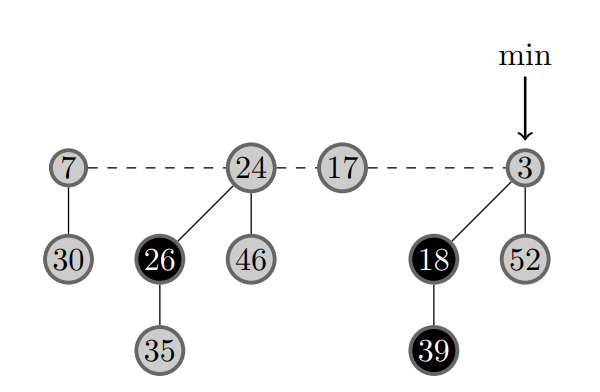
\includegraphics[width=\textwidth]{e1.png}
         \caption{}
         \label{fig:e1}
     \end{subfigure}
     \hspace*{\fill}
    %---------fig 2-------
    \begin{subfigure}[H]{0.5\linewidth}
         \centering
         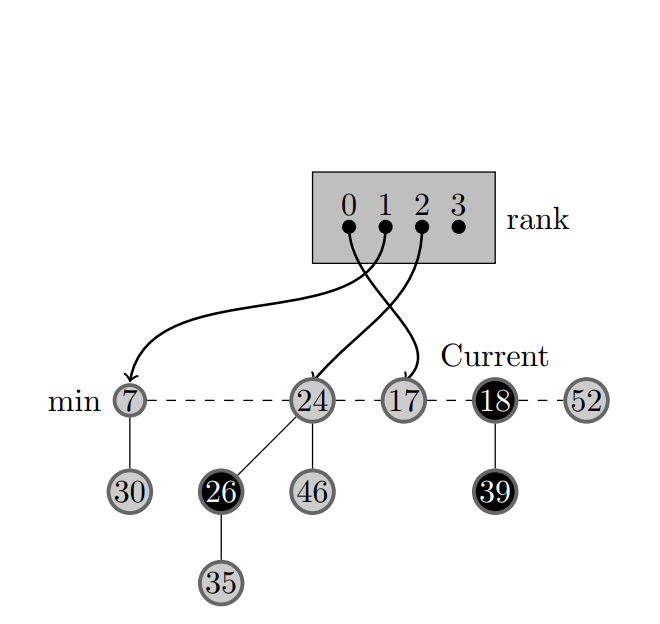
\includegraphics[width=\textwidth]{e2.png}
         \caption{}
         \label{fig:e2}
     \end{subfigure}
 %---------fig 3-------
\begin{subfigure}[H]{0.4\textwidth}
         \centering
         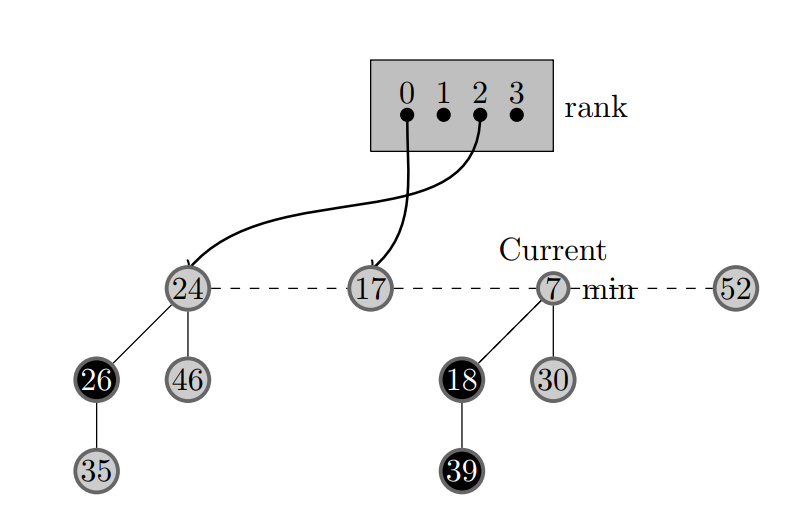
\includegraphics[width=\textwidth]{e3.png}
         \caption{}
         \label{fig:e3}
     \end{subfigure}
     \hspace*{\fill}
 %---------fig 4-------
\begin{subfigure}[H]{0.4\textwidth}
         \centering
         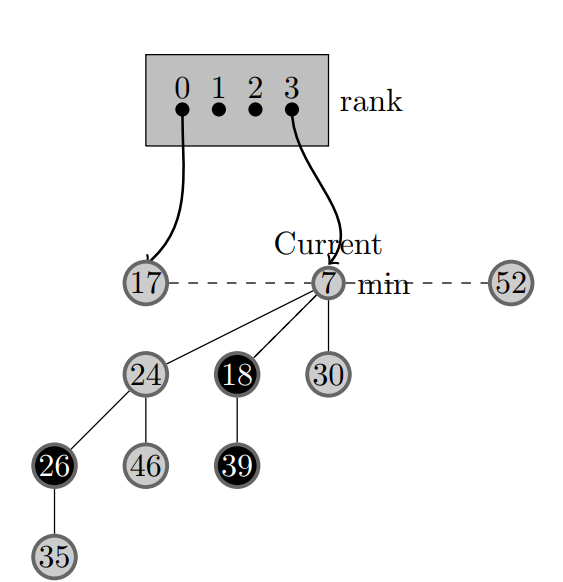
\includegraphics[width=\textwidth]{e4.png}
         \caption{}
         \label{fig:e4}
     \end{subfigure}
     
 
 %---------fig 5-------
\begin{subfigure}[H]{0.4\textwidth}
         \centering
         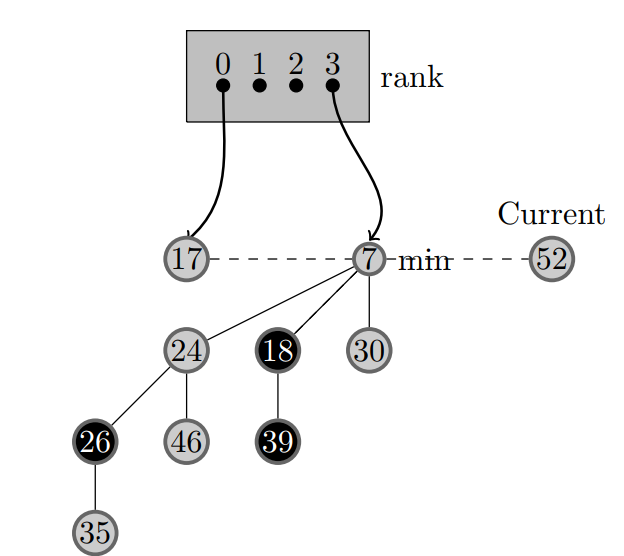
\includegraphics[width=\textwidth]{e5.png}
         \caption{}
         \label{fig:e4}
     \end{subfigure}
     \hspace*{\fill}
 %---------fig 6-------
\begin{subfigure}[H]{0.4\textwidth}
         \centering
         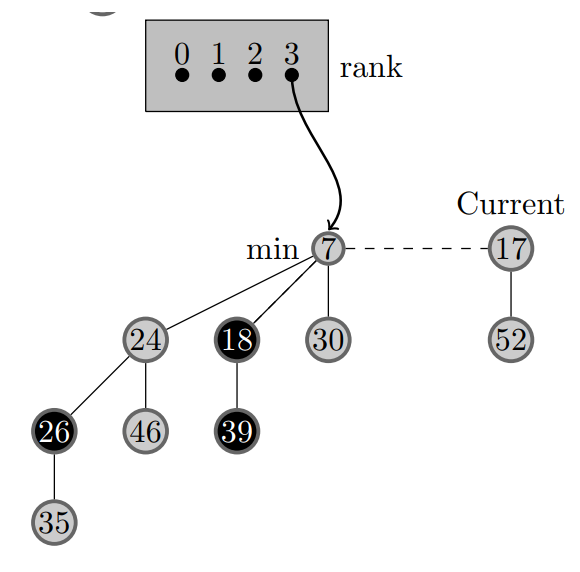
\includegraphics[width=\textwidth]{e6.png}
         \caption{}
         \label{fig:e6}
     \end{subfigure}

 %---------fig 7-------
\begin{subfigure}[H]{0.4\textwidth}
         \centering
         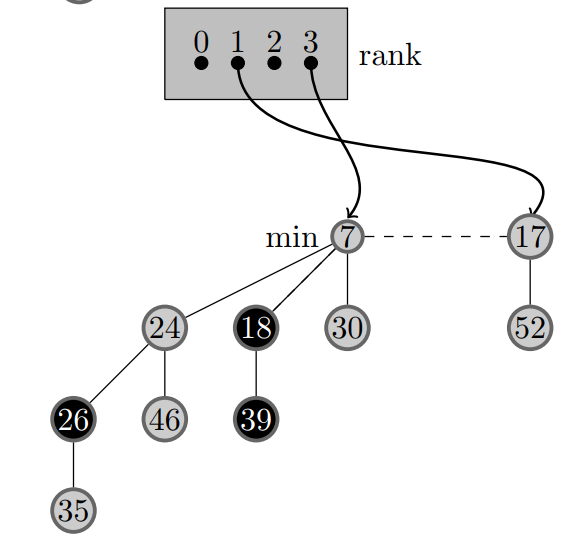
\includegraphics[width=\textwidth]{e7.png}
         \caption{}
         \label{fig:e7}
     \end{subfigure}
    \caption{Extract min}
    \label{fig:e}
\end{figure}



% \begin{tikzpicture}[
% roundnode/.style={circle, draw=black!60, fill=black!20, very thick, minimum size=1mm, inner sep=1pt,}
% ]
%  \node [roundnode] (a1) at (0, 0)  { 7 };
%  \node [roundnode] (a2) at (0,-1) { 30 };
 
% \node [roundnode] (b1) at (2, 0) { 24 };
% \node [roundnode] (b2) at (2,-1) { 46 };
% \node [roundnode,fill=black,text=white] (b3) at (1,-1) { 26 };
% \node [roundnode] (b4) at (1,-2) { 35 };

% \node [roundnode] (c) at (3, 0) { 17 };

% \node [roundnode] (d1) at (5, 0)  { 3 };
% \node [roundnode] (d2) at (5,-1) { 52 };
% \node [roundnode,fill=black,text=white] (d3) at (4,-1) { 18 };
% \node [roundnode,fill=black,text=white] (d4) at (4,-2) { 39 };
% % \node [roundnode] (d5) at (7,-1) { 41 };
% % \node [roundnode] (d6) at (7,-2) { 44 };
% \draw (a1) edge (a2);
% \draw [dashed](a1) edge (b1);
% \draw (b1) edge (b2);
% \draw (b1) edge (b3);
% \draw (b3) edge (b4);

% \draw [dashed] (b1) edge (c);

% \draw [dashed] (c) edge (d1);
% \draw (d1) edge (d2);
% \draw (d1) edge (d3);
% % \draw (d1) edge (d5);
% \draw (d3) edge (d4);
% % \draw (d5) edge (d6);
% \draw [thick,->](5,1) node[above]{min} to (5,0.3);

% \end{tikzpicture}



% \hspace{1cm}
% \begin{tikzpicture}[
% roundnode/.style={circle, draw=black!60, fill=black!20, very thick, minimum size=1mm, inner sep=0.5pt,}
% ]
%     %Block er rank er track
%     \draw [fill=gray!50] (2,1.5) -- (4,1.5) -- node[right] {rank}(4,2.5) -- (2,2.5) -- (2,1.5);
%     \filldraw [black,xshift=2.4cm, yshift=1.9cm,label=0] (0,0) circle  (2pt) node[above] {0};
%     \filldraw [black,xshift=2.8cm, yshift=1.9cm] (0,0) circle (2pt)node[above] {1};
%     \filldraw [black,xshift=3.2cm, yshift=1.9cm] (0,0) circle (2pt)node[above] {2};
%     \filldraw [black,xshift=3.6cm, yshift=1.9cm] (0,0) circle (2pt)node[above] {3};
    
%     \draw[thick,->] (2.8,1.9)  to[out=-90,in=90]    (0,0.2) ;
    
%      %nodes
%      \node [roundnode,label=left:min,label=above:Current] (a1) at (0, 0)  { 7 };
%      \node [roundnode] (a2) at (0,-1) { 30 };


%     \node [roundnode] (b1) at (2, 0) { 24 };
%     \node [roundnode] (b2) at (2,-1) { 46 };
%     \node [roundnode,fill=black,text=white] (b3) at (1,-1) { 26 };
%     \node [roundnode] (b4) at (1,-2) { 35 };
    
%     \node [roundnode] (c) at (3, 0) { 17 };
    
%     \node [roundnode,fill=black,text=white] (d1) at (4, 0)  { 18 };
%     \node [roundnode,fill=black,text=white] (d2) at (4,-1) { 39 };
    
%     \node [roundnode] (e) at (5,0) { 52 };

%     \draw (a1) edge (a2);
%     \draw[dashed] (a1) edge (b1);
%     \draw (b1) edge (b2);
%     \draw (b1) edge (b3);
%     \draw (b3) edge (b4);
    
%     \draw [dashed] (b1) edge (c);
    
%     \draw[dashed] (c) edge (d1);
%     \draw  (d1) edge (d2);
    
%     \draw[dashed] (d1) edge (e);
% \end{tikzpicture}
% \vspace{1.5cm}\\
% \begin{tikzpicture}[
% roundnode/.style={circle, draw=black!60, fill=black!20, very thick, minimum size=1mm, inner sep=0.5pt,}
% ]
%     %Block er rank er track
%     \draw [fill=gray!50] (2,1.5) -- (4,1.5) -- node[right] {rank}(4,2.5) -- (2,2.5) -- (2,1.5);
%     \filldraw [black,xshift=2.4cm, yshift=1.9cm,label=0] (0,0) circle  (2pt) node[above] {0};
%     \filldraw [black,xshift=2.8cm, yshift=1.9cm] (0,0) circle (2pt)node[above] {1};
%     \filldraw [black,xshift=3.2cm, yshift=1.9cm] (0,0) circle (2pt)node[above] {2};
%     \filldraw [black,xshift=3.6cm, yshift=1.9cm] (0,0) circle (2pt)node[above] {3};

%     \draw[thick,->] (2.8,1.9)  to[out=-90,in=80]    (0,0.2) ;
%     \draw[thick,->] (3.2,1.9)  to[out=-90,in=50]    (2,0.2) ;
%     \draw[thick,->] (2.4,1.9)  to[out=-90,in=40]    (3,0.2) ;
    
         
%      %nodes
%      \node [roundnode,label=left:min] (a1) at (0, 0)  { 7 };
%      \node [roundnode] (a2) at (0,-1) { 30 };


%     \node [roundnode] (b1) at (2, 0) { 24 };
%     \node [roundnode] (b2) at (2,-1) { 46 };
%     \node [roundnode,fill=black,text=white] (b3) at (1,-1) { 26 };
%     \node [roundnode] (b4) at (1,-2) { 35 };
    
%     \node [roundnode] (c) at (3, 0) { 17 };
    
%     \node [roundnode,fill=black,text=white,label=above:Current] (d1) at (4, 0)  { 18 };
%     \node [roundnode,fill=black,text=white] (d2) at (4,-1) { 39 };
    
%     \node [roundnode] (e) at (5,0) { 52 };
    
%     \draw (a1) edge (a2);
%     \draw[dashed] (a1) edge (b1);
%     \draw (b1) edge (b2);
%     \draw (b1) edge (b3);
%     \draw (b3) edge (b4);
    
%     \draw [dashed] (b1) edge (c);
    
%     \draw[dashed] (c) edge (d1);
%     \draw  (d1) edge (d2);
    
%     \draw[dashed] (d1) edge (e);
%     % \draw[dashed] (e) edge (f1);
%     % \draw (f1) edge (f2);
% \end{tikzpicture}
% \hspace{1cm}
% \begin{tikzpicture}[
% roundnode/.style={circle, draw=black!60, fill=black!20, very thick, minimum size=1mm, inner sep=0.5pt,}
% ]
%     %Block er rank er track
%     \draw [fill=gray!50] (4,1.5) -- (6,1.5) -- node[right] {rank}(6,2.5) -- (4,2.5) -- (4,1.5);
%     \filldraw [black,xshift=4.4cm, yshift=1.9cm,label=0] (0,0) circle  (2pt) node[above] {0};
%     \filldraw [black,xshift=4.8cm, yshift=1.9cm] (0,0) circle (2pt)node[above] {1};
%     \filldraw [black,xshift=5.2cm, yshift=1.9cm] (0,0) circle (2pt)node[above] {2};
%     \filldraw [black,xshift=5.6cm, yshift=1.9cm] (0,0) circle (2pt)node[above] {3};

%     \draw[thick,->] (5.2,1.9)  to[out=-90,in=50]    (2,0.2) ;
%     \draw[thick,->] (4.4,1.9)  to[out=-90,in=40]    (4,0.2) ;
    
%      %nodes
     
%     \node [roundnode] (b1) at (2, 0) { 24 };
%     \node [roundnode] (b2) at (2,-1) { 46 };
%     \node [roundnode,fill=black,text=white] (b3) at (1,-1) { 26 };
%     \node [roundnode] (b4) at (1,-2) { 35 };
    
%     \node [roundnode] (c) at (4, 0) { 17 };
    
%     \node [roundnode,label=right:min,label=above:Current] (a1) at (6, 0)  { 7 };
%      \node [roundnode] (a2) at (6,-1) { 30 };
%     \node [roundnode,fill=black,text=white] (d1) at (5, -1)  { 18 };
%     \node [roundnode,fill=black,text=white] (d2) at (5,-2) { 39 };
    
%     \node [roundnode] (e) at (8,0) { 52 };
    
%     \draw (a1) edge (a2);
    
%     \draw (b1) edge (b2);
%     \draw (b1) edge (b3);
%     \draw (b3) edge (b4);
    
%     \draw [dashed] (b1) edge (c);
%     \draw [dashed] (c) edge (a1);
    
%     \draw[dashed] (a1) edge (d1);
%     \draw  (d1) edge (d2);
%     \draw  (a1) edge (d1);
    
%     \draw[dashed] (a1) edge (e);
% \end{tikzpicture}
% \vspace{0.3cm}\\

% \begin{tikzpicture}[
% roundnode/.style={circle, draw=black!60, fill=black!20, very thick, minimum size=1mm, inner sep=0.5pt,}
% ]
%     %Block er rank er track
%     \draw [fill=gray!50] (4,1.5) -- (6,1.5) -- node[right] {rank}(6,2.5) -- (4,2.5) -- (4,1.5);
%     \filldraw [black,xshift=4.4cm, yshift=1.9cm,label=0] (0,0) circle  (2pt) node[above] {0};
%     \filldraw [black,xshift=4.8cm, yshift=1.9cm] (0,0) circle (2pt)node[above] {1};
%     \filldraw [black,xshift=5.2cm, yshift=1.9cm] (0,0) circle (2pt)node[above] {2};
%     \filldraw [black,xshift=5.6cm, yshift=1.9cm] (0,0) circle (2pt)node[above] {3};

%     \draw[thick,->] (5.6,1.9)  to[out=-90,in=50]    (6,0.2) ;
%     \draw[thick,->] (4.4,1.9)  to[out=-90,in=40]    (4,0.2) ;
    
         
%      %nodes
     
    
%     \node [roundnode] (c) at (4, 0) { 17 };
    
%     \node [roundnode,label=right:min,label=above:Current] (a1) at (6, 0)  { 7 };
%      \node [roundnode] (a2) at (6,-1) { 30 };
%     \node [roundnode,fill=black,text=white] (d1) at (5, -1)  { 18 };
%     \node [roundnode,fill=black,text=white] (d2) at (5,-2) { 39 };
%      \node [roundnode] (b1) at (4, -1) { 24 };
%     \node [roundnode] (b2) at (4,-2) { 46 };
%     \node [roundnode,fill=black,text=white] (b3) at (3,-2) { 26 };
%     \node [roundnode] (b4) at (3,-3) { 35 };
    
%     \node [roundnode] (e) at (8,0) { 52 };
%     \draw (a1) edge (a2);
    
%     \draw (b1) edge (b2);
%     \draw (b1) edge (b3);
%     \draw (b3) edge (b4);
    
%     \draw [dashed] (c) edge (a1);
    
%     \draw[dashed] (a1) edge (d1);
%     \draw (a1) edge (b1);
%     \draw  (d1) edge (d2);
%     \draw  (a1) edge (d1);
    
%     \draw[dashed] (a1) edge (e);
% \end{tikzpicture}
% \hspace{1cm}
% \begin{tikzpicture}[
% roundnode/.style={circle, draw=black!60, fill=black!20, very thick, minimum size=1mm, inner sep=0.5pt,}
% ]
%     %Block er rank er track
%     \draw [fill=gray!50] (4,1.5) -- (6,1.5) -- node[right] {rank}(6,2.5) -- (4,2.5) -- (4,1.5);
%     \filldraw [black,xshift=4.4cm, yshift=1.9cm,label=0] (0,0) circle  (2pt) node[above] {0};
%     \filldraw [black,xshift=4.8cm, yshift=1.9cm] (0,0) circle (2pt)node[above] {1};
%     \filldraw [black,xshift=5.2cm, yshift=1.9cm] (0,0) circle (2pt)node[above] {2};
%     \filldraw [black,xshift=5.6cm, yshift=1.9cm] (0,0) circle (2pt)node[above] {3};

%     \draw[thick,->] (5.6,1.9)  to[out=-90,in=50]    (6,0.2) ;
%     \draw[thick,->] (4.4,1.9)  to[out=-90,in=40]    (4,0.2) ;
    
         
%      %nodes
     
    
%     \node [roundnode] (c) at (4, 0) { 17 };
    
%     \node [roundnode,label=right:min] (a1) at (6, 0)  { 7 };
%      \node [roundnode] (a2) at (6,-1) { 30 };
%     \node [roundnode,fill=black,text=white] (d1) at (5, -1)  { 18 };
%     \node [roundnode,fill=black,text=white] (d2) at (5,-2) { 39 };
%      \node [roundnode] (b1) at (4, -1) { 24 };
%     \node [roundnode] (b2) at (4,-2) { 46 };
%     \node [roundnode,fill=black,text=white] (b3) at (3,-2) { 26 };
%     \node [roundnode] (b4) at (3,-3) { 35 };
    
%     \node [roundnode,label=above:Current] (e) at (8,0) { 52 };
%     \draw (a1) edge (a2);
    
%     \draw (b1) edge (b2);
%     \draw (b1) edge (b3);
%     \draw (b3) edge (b4);
    
%     \draw [dashed] (c) edge (a1);
    
%     \draw[dashed] (a1) edge (d1);
%     \draw (a1) edge (b1);
%     \draw  (d1) edge (d2);
%     \draw  (a1) edge (d1);
    
%     \draw[dashed] (a1) edge (e);
% \end{tikzpicture}
% \vspace{0.5cm}
% \begin{tikzpicture}[
% roundnode/.style={circle, draw=black!60, fill=black!20, very thick, minimum size=1mm, inner sep=0.5pt,}
% ]
%     %Block er rank er track
%     \draw [fill=gray!50] (4,1.5) -- (6,1.5) -- node[right] {rank}(6,2.5) -- (4,2.5) -- (4,1.5);
%     \filldraw [black,xshift=4.4cm, yshift=1.9cm,label=0] (0,0) circle  (2pt) node[above] {0};
%     \filldraw [black,xshift=4.8cm, yshift=1.9cm] (0,0) circle (2pt)node[above] {1};
%     \filldraw [black,xshift=5.2cm, yshift=1.9cm] (0,0) circle (2pt)node[above] {2};
%     \filldraw [black,xshift=5.6cm, yshift=1.9cm] (0,0) circle (2pt)node[above] {3};

%     \draw[thick,->] (5.6,1.9)  to[out=-90,in=50]    (6,0.2) ;
         
%      %nodes
     
    
%     \node [roundnode,label=left:min] (a1) at (6, 0)  { 7 };
%      \node [roundnode] (a2) at (6,-1) { 30 };
%     \node [roundnode,fill=black,text=white] (d1) at (5, -1)  { 18 };
%     \node [roundnode,fill=black,text=white] (d2) at (5,-2) { 39 };
%      \node [roundnode] (b1) at (4, -1) { 24 };
%     \node [roundnode] (b2) at (4,-2) { 46 };
%     \node [roundnode,fill=black,text=white] (b3) at (3,-2) { 26 };
%     \node [roundnode] (b4) at (3,-3) { 35 };
    
%      \node [roundnode,label=above:Current] (c) at (8, 0) { 17 };
%     \node [roundnode] (e) at (8,-1) { 52 };
    
%     % \node [roundnode] (f1) at (10,0) { 41 };
%     % \node [roundnode] (f2) at (10,-1) { 44 };
%     \draw (a1) edge (a2);
    
%     \draw (b1) edge (b2);
%     \draw (b1) edge (b3);
%     \draw (b3) edge (b4);

    
%     \draw[dashed] (a1) edge (d1);
%     \draw (a1) edge (b1);
%     \draw  (d1) edge (d2);
%     \draw  (a1) edge (d1);
    
%     \draw  (c) edge (e);
%     \draw[dashed] (a1) edge (c);
%     % \draw[dashed] (c) edge (f1);
%     % \draw (f1) edge (f2);
% \end{tikzpicture}
% \hspace{1cm}
% \begin{tikzpicture}[
% roundnode/.style={circle, draw=black!60, fill=black!20, very thick, minimum size=1mm, inner sep=0.5pt,}
% ]
%     %Block er rank er track
%   \draw [fill=gray!50] (4,1.5) -- (6,1.5) -- node[right] {rank}(6,2.5) -- (4,2.5) -- (4,1.5);
%     \filldraw [black,xshift=4.4cm, yshift=1.9cm,label=0] (0,0) circle  (2pt) node[above] {0};
%     \filldraw [black,xshift=4.8cm, yshift=1.9cm] (0,0) circle (2pt)node[above] {1};
%     \filldraw [black,xshift=5.2cm, yshift=1.9cm] (0,0) circle (2pt)node[above] {2};
%     \filldraw [black,xshift=5.6cm, yshift=1.9cm] (0,0) circle (2pt)node[above] {3};

%     \draw[thick,->] (5.6,1.9)  to[out=-90,in=50]    (6,0.2) ;

%     \draw[thick,->] (4.8,1.9)  to[out=-90,in=50]    (8,0.2) ;
         
%      %nodes
     
    
%     \node [roundnode,label=left:min] (a1) at (6, 0)  { 7 };
%      \node [roundnode] (a2) at (6,-1) { 30 };
%     \node [roundnode,fill=black,text=white] (d1) at (5, -1)  { 18 };
%     \node [roundnode,fill=black,text=white] (d2) at (5,-2) { 39 };
%      \node [roundnode] (b1) at (4, -1) { 24 };
%     \node [roundnode] (b2) at (4,-2) { 46 };
%     \node [roundnode,fill=black,text=white] (b3) at (3,-2) { 26 };
%     \node [roundnode] (b4) at (3,-3) { 35 };
    
%      \node [roundnode] (c) at (8, 0) { 17 };
%     \node [roundnode] (e) at (8,-1) { 52 };
    
%     % \node [roundnode] (f1) at (10,0) { 41 };
%     % \node [roundnode] (f2) at (10,-1) { 44 };
%     \draw (a1) edge (a2);
    
%     \draw (b1) edge (b2);
%     \draw (b1) edge (b3);
%     \draw (b3) edge (b4);

    
%     \draw[dashed] (a1) edge (d1);
%     \draw (a1) edge (b1);
%     \draw  (d1) edge (d2);
%     \draw  (a1) edge (d1);
    
%     \draw  (c) edge (e);
%     \draw[dashed] (a1) edge (c);
%     % \draw[dashed] (c) edge (f1);
%     % \draw (f1) edge (f2);
% \end{tikzpicture}
\subsection{Delete}
To delete any node from fibonacci heap, previous two operation are applied. These are -\\
\begin{enumerate}
    \item We decrease key
    \item We extract min
\end{enumerate}
Following algorithm is followed-\\
\begin{enumerate}
    \item We decrease the node to minus infinity.
    \item We bring the node into the root list by heapifying the heap containing the minus infinity.
    \item We perform the extract min operation.
\end{enumerate}
\textbf{Running time of decrease key : O(1)}\\
\textbf{Running time of extract min : O(logn)}\\ \\

\textbf{Running time of Delete key : O(logn)}\\ \\ 
\hspace{-0.7cm}Example-\\[0.5cm]
\begin{tikzpicture}[
roundnode/.style={circle, draw=black!60, fill=black!20, very thick, minimum size=5mm, inner sep=1pt,}
]
    \node[roundnode] (a1) at (0,0){7};
    \node[roundnode] (a2) at (0,-1){9};
    
    \node[roundnode,label=above:min] (b1) at (2,0){2};
    \node[roundnode] (b2) at (2,-1){3};
    \node[roundnode] (b3) at (1,-1){4};
    \node[roundnode] (b4) at (1,-2){5};
    
    \draw[dashed] (a1) edge (b1);
    \draw (a1) edge (a2);
    
    \draw (b1) edge (b2);
    \draw (b1) edge (b3);
    \draw (b3) edge (b4);
    
    \draw[->] (3,-1) --node[above]{ 5 to $-\infty$} (4.5,-1);
\end{tikzpicture}
\begin{tikzpicture}[
roundnode/.style={circle, draw=black!60, fill=black!20, very thick, minimum size=5mm, inner sep=1pt,}
]
    \node[roundnode] (a1) at (0,0){7};
    \node[roundnode] (a2) at (0,-1){9};
    
    \node[roundnode,label=above:min] (b1) at (2,0){$-\infty$};
    \node[roundnode] (b2) at (2,-1){3};
    \node[roundnode] (b3) at (1,-1){2};
    \node[roundnode] (b4) at (1,-2){4};
    
    \draw[dashed] (a1) edge (b1);
    \draw (a1) edge (a2);
    
    \draw (b1) edge (b2);
    \draw (b1) edge (b3);
    \draw (b3) edge (b4);
    
    \draw[->] (3,-1) --node[above]{extract min} (5,-1);
\end{tikzpicture}	
\begin{tikzpicture}[
roundnode/.style={circle, draw=black!60, fill=black!20, very thick, minimum size=5mm, inner sep=1pt,}
]
    \node[roundnode] (a1) at (0,0){3};
    
    \node[roundnode,label=above:min] (b1) at (2,0){2};
    \node[roundnode] (b2) at (2,-1){4};
    \node[roundnode] (b3) at (1,-1){7};
    \node[roundnode] (b4) at (1,-2){9};
    
    \draw[dashed] (a1) edge (b1);
    
    \draw (b1) edge (b2);
    \draw (b1) edge (b3);
    \draw (b3) edge (b4);
\end{tikzpicture}
\subsection{Find min}
Finding minimum is easy in fibonacci heap. Minimum element is always given by Min pointer. So this operation takes constant time.\\[0.5cm]
\textbf{Running time of Find Min : O(1)}
\section{Maximally Damaged tree}
Binomial heap with order k has $2^{k}$ number of nodes. But in fibonacci heap $2^{k}$ property are not satisfied always.When we cut the children in fibonacci heap, $2^{k}$ property does not apply on fibonacci heap.\\
If a tree does not grow with height, height does not remain logn. After cutting a children in fibonacci heap, we want to show that fibonacci tree with k height has $c^{k}$ nodes where $c>1$. we do not want to delete too many nodes from a tree, as we still want a tree of rank k to have $c^{k}$ nodes. The reason for wanting this property is so that the searching part of delete-min should take only O(log n) steps. 
\\
Here is an example of tree with rank 5. We will cut its higher degree nodes without cutting the root node.
\begin{figure}[h]
    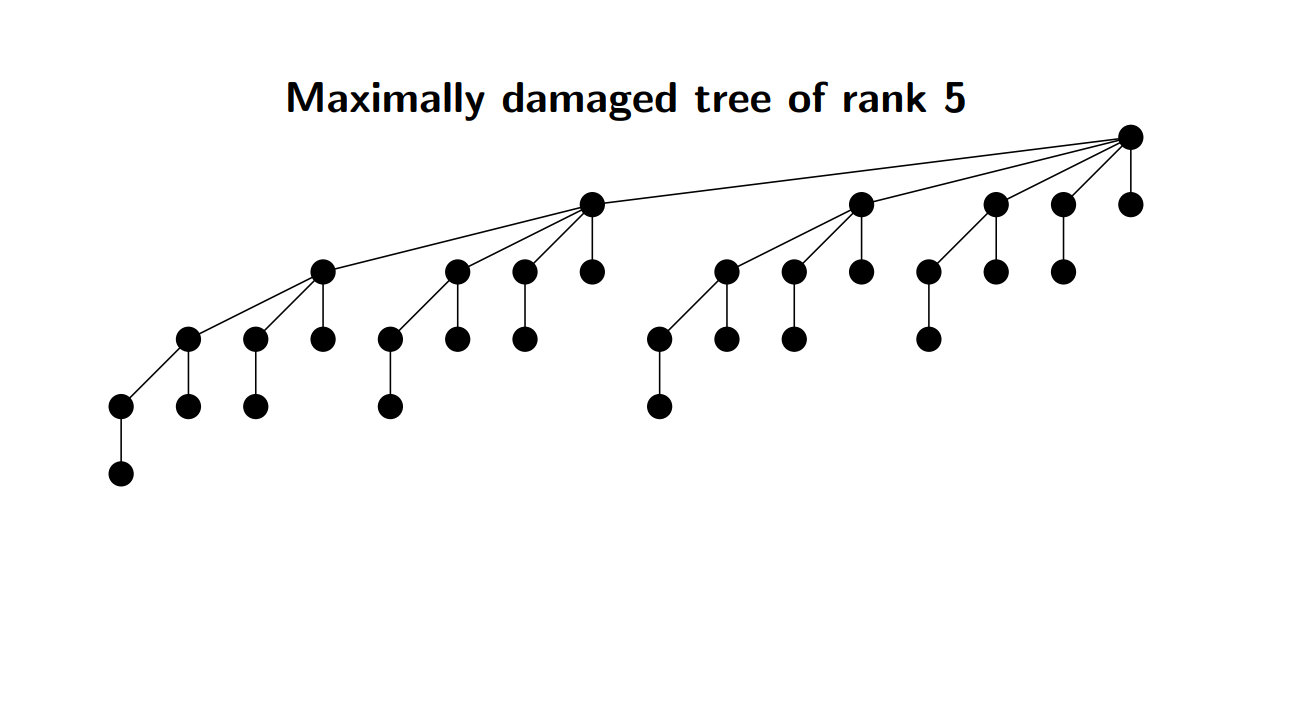
\includegraphics[scale=.3,bb=0 0 404 401]{1.png}
    \caption{Binomial tree of rank 5}
    \label{fig:one}
\end{figure}
\begin{figure}[H]
    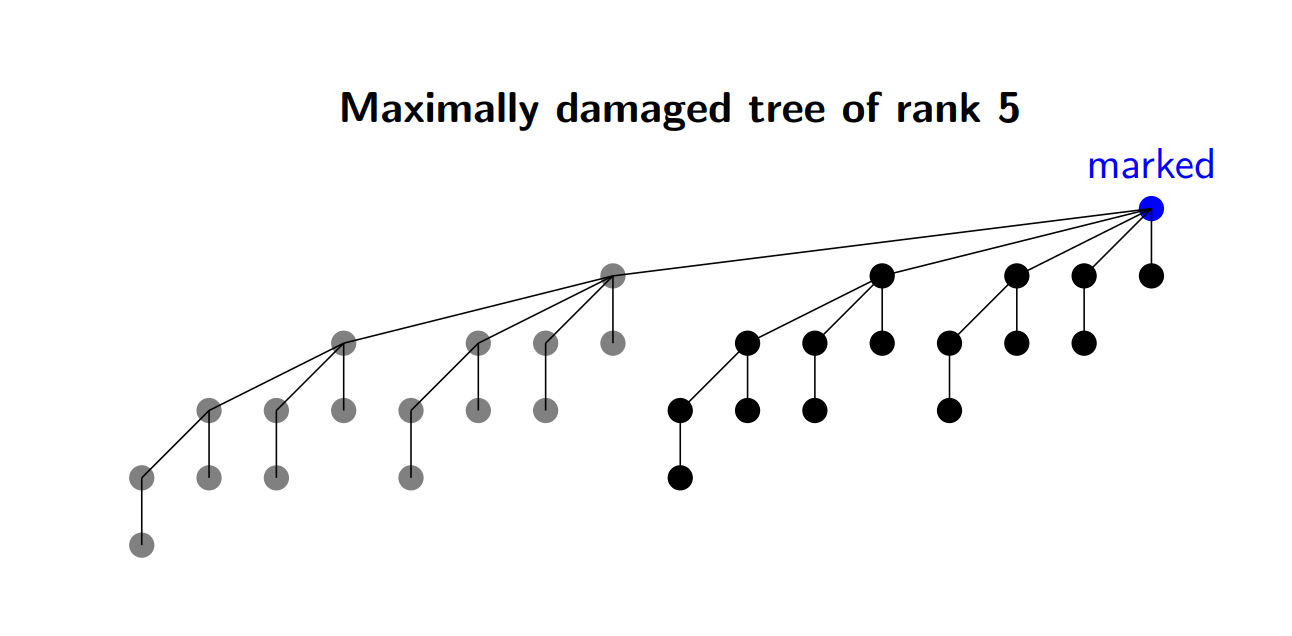
\includegraphics[scale=.3,bb=0 0 404 401]{2.png}
    \caption{}
    \label{fig:two}
\end{figure}
\begin{figure}[H]
    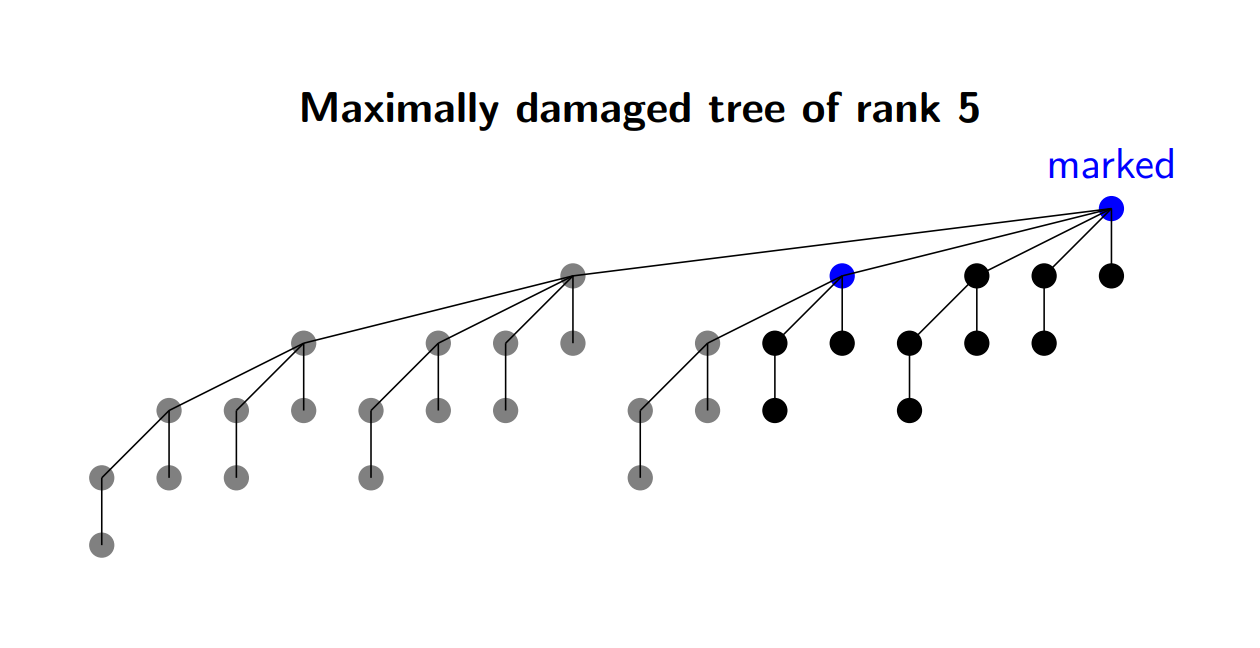
\includegraphics[scale=.3,bb=0 0 404 401]{3.png}
    \caption{}
    \label{fig:three}
\end{figure}
\begin{figure}[H]
    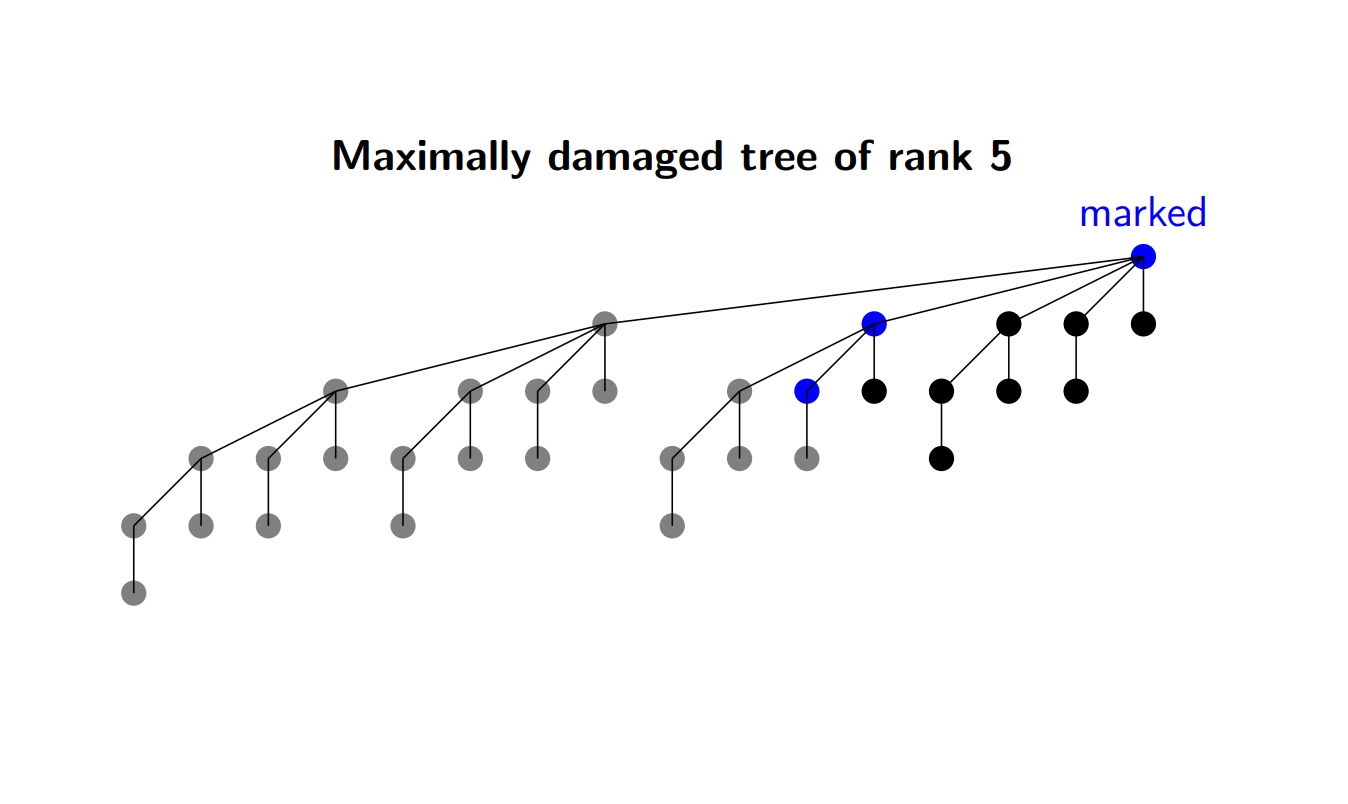
\includegraphics[scale=.3,bb=0 0 404 401]{4.png}
    \caption{}
    \label{fig:four}
\end{figure}
\begin{figure}[H]
    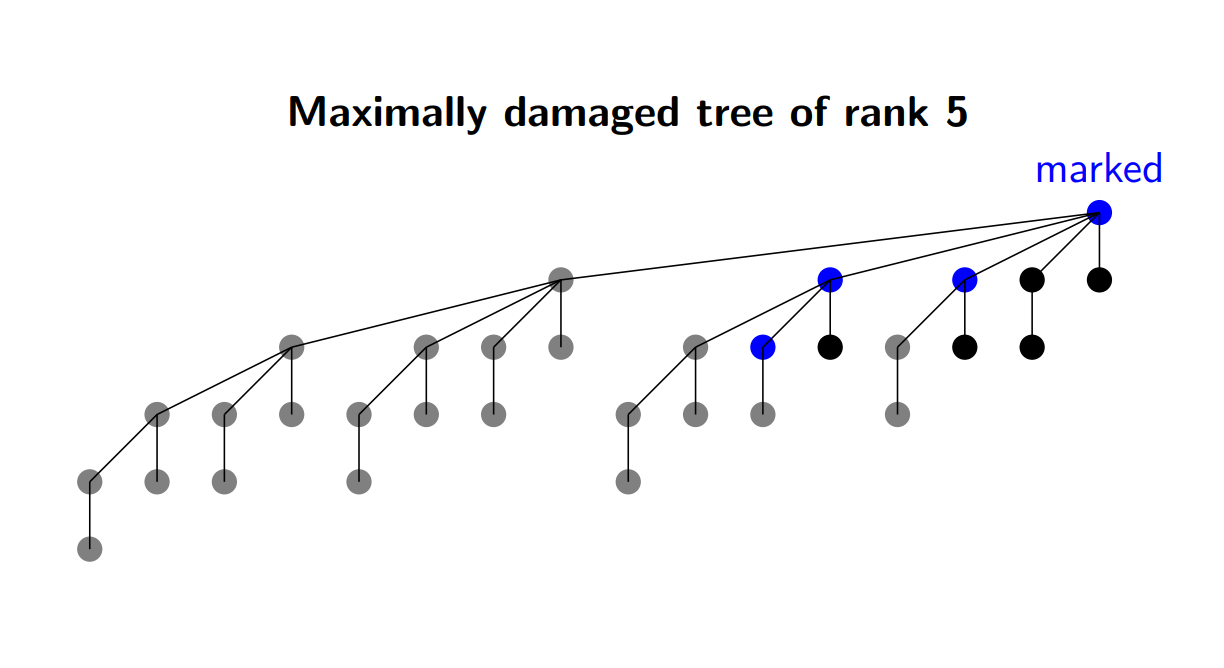
\includegraphics[scale=.3,bb=0 0 404 401]{5.png}
    \caption{}
    \label{fig:five}
\end{figure}
\begin{figure}[H]
    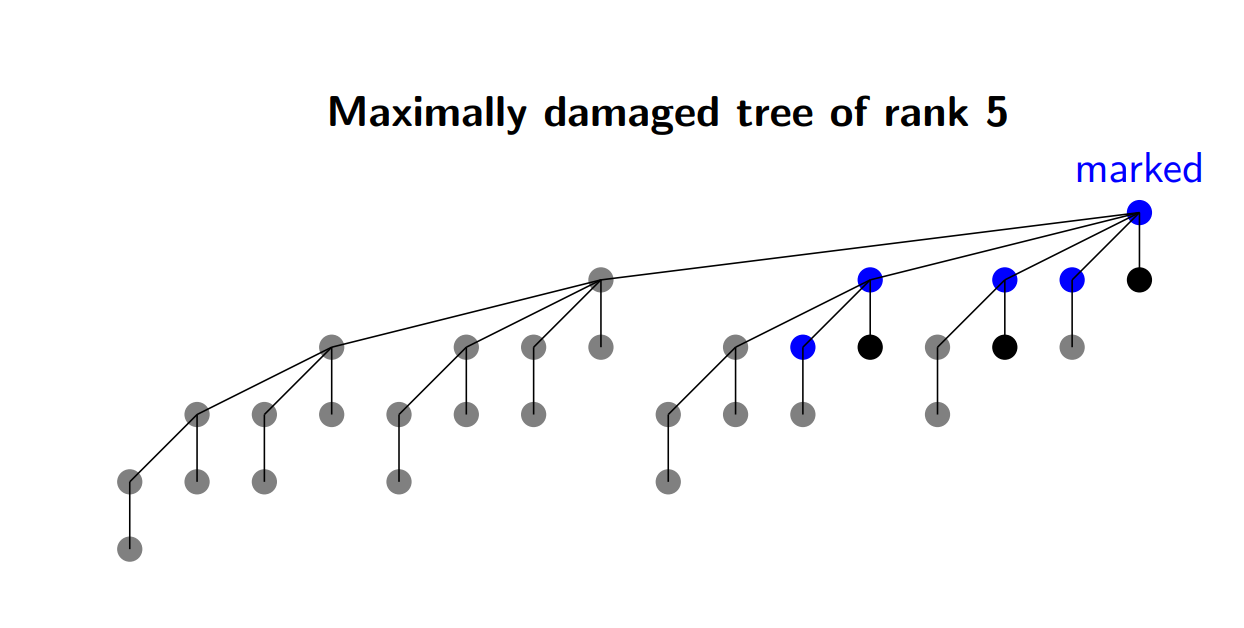
\includegraphics[scale=.3,bb=0 0 404 401]{6.png}
    \caption{}
    \label{fig:six}
\end{figure}
\vspace{1cm}
So this is the maximally damaged tree with rank 5.This is a fibonacci tree. This tree has $c^k$ number of node where c$>$1 and $c<2$. If we damaged binomial tree with different rank , we will get fibonacci tree corrresponding to the binomial tree.
\begin{figure}[H]
    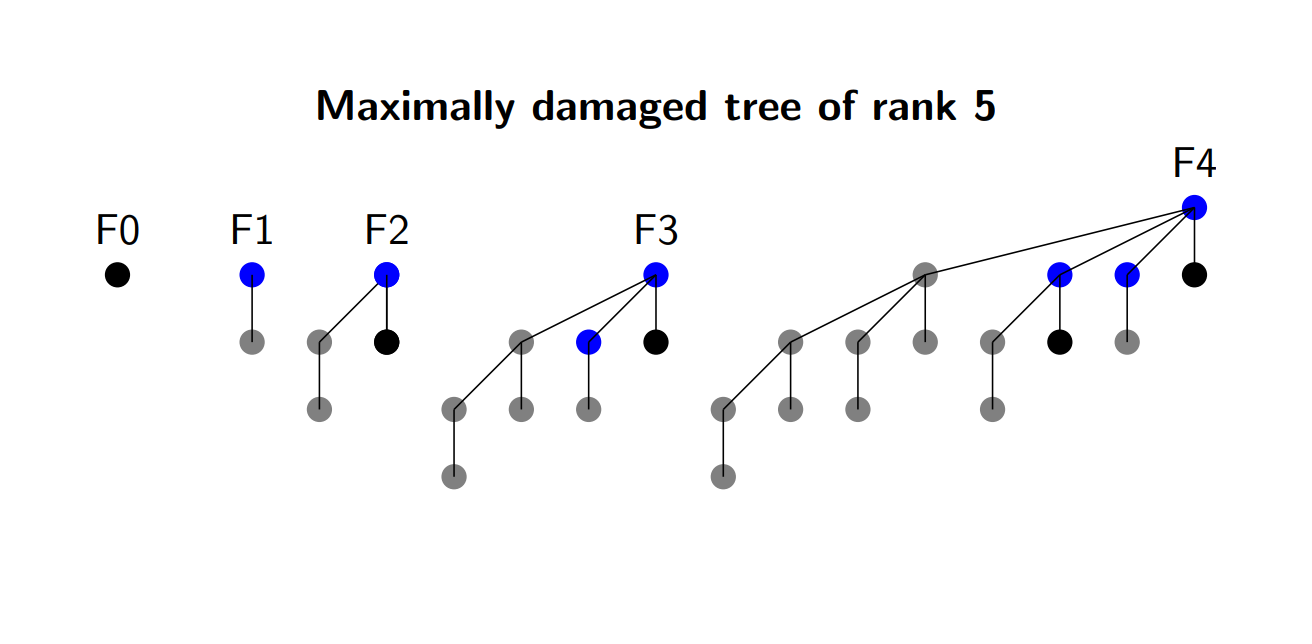
\includegraphics[scale=.3,bb=0 0 404 401]{7.png}
    \caption{}
    \label{fig:six}
\end{figure}
In Figure 21 , we can see the formation of fibonacci tree. Current tree is consist of its first and second preceding. This is like fibonacci number series.That is why this heap is called fibonacci heap.\\
\begin{figure}[H]
    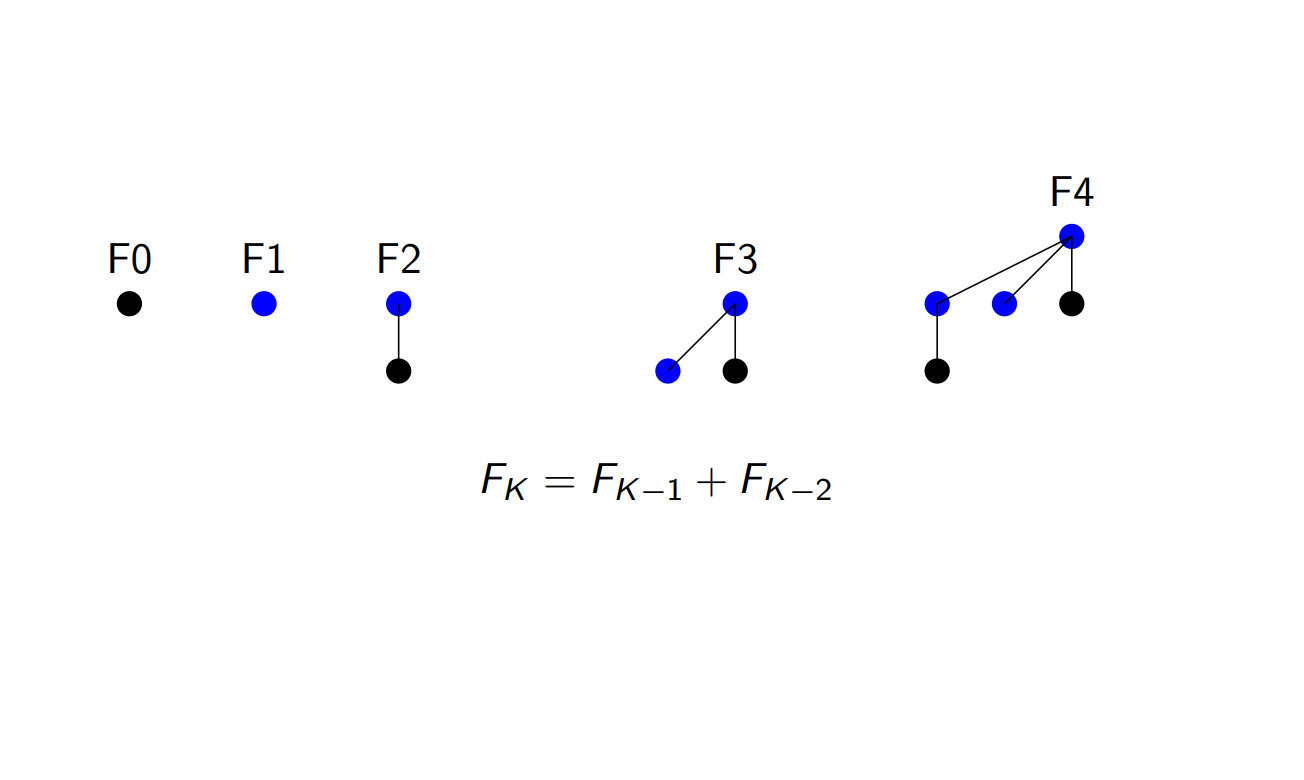
\includegraphics[scale=.3,bb=0 0 400 401]{8.png}
    \caption{}
    \label{fig:six}
\end{figure}
\bigskip
\hspace{-0.65cm}
Size of $f_k$ is: $S_{k} >= c^{k}$ \\
Fibonacci trees still grow exponentially fast in k.\\
$$c= (1+\sqrt{5})/2$$
rank = O($log_{c} k$) = O($log n$)

% \pagebreak
\section{Amortized Running time}
Amortized running time is a method to compute complexity of an algorithm. Amortized running time is that looking at the worst running time per operation.
Here is an example of amortized running time -\\
If a number of insertion, b number of decrease key and c number of extract min are taken,\\ the amortized running time :
\textbf{O(a+b+clogn)}\\[0.5cm]
\chapter{Conclusion}
\par
Heaps have a variety of application in network optimization and in many such applications. Thus Fibonacci heap is also faster for several well-known network optimization problems. Purpose of fibonacci heap is to speed up Dijkstra's algorithm for single source shortest path problem with non negative edges.Now Djkstra's algorithm runs O(nlogn+m) improved from $O(mlog_{m/n+2}n)$\cite{one}.\\
Various other network use Dijkstra's algorithm as a subroutine and for each of these, we obtain a corresponding improvement.
\\[0.5cm]
\begin{thebibliography}{9}
\bibitem{one} 
Michael L. Fredman and Robert Endree Tarjan.
\textit{"Fibonacci Heaps and Their Uses in Improved Network Optimization Algorithms"}. Journal of the ACM, 34(3):596-615, 1987.
\end{thebibliography}
\end{document}
